
%\chapter{Objectives}

\chapter{Context}

\section{Global change: how to describe the future of alpine ecosystems?}

\subsection{The value of ecosystems: from properties to services}

\paragraph{A new logic}
Everyone has a particular relationship with nature. The representation of the nature depends on the way we experienced it -- temperate or tropical forests, mountain rivers or cliffs on the ocean littoral, bird songs or wind between stones. Anyone who shares one of these visions will likely want to preserve natural systems. But facing this emotional perception and inner desire to see these ecosystems preserved, there are other forces that push in opposite directions. All indexes of the biodiversity decrease at dangerous rates \parencite{butchart_global_2010}, despite increasing local efforts and positive effect of conservation fundings \parencite{waldron_reductions_2017}, the deforestation threatens the largest forest systems, insects are less and less presents \parencite{hallmann_more_2017} and animals are repelled to fragmented and diminishing habitats \parencite{tucker_moving_2018}. Logics, other than emotional attachment and will to protect nature, impact all natural systems around the world because they are driven by other interests. To be protected, the natural systems needed a way to be integrated within these strong driving logics. The notion of \textemph{ecosystem services}\sidenote{highlighted terms correspond to key terms and are listed in the index at the end of this document.} was developed by \cite{costanza_value_1997} to capture the value of \textemph{ecosystems}. It encompasses the benefits humans extract from ecosystems. It enables a categorisation of services and their quantification (up to the level of the monetisation), and therefore allows them to be taken into consideration in the global logic of capital, investment and value.


\paragraph{Services}
The notion of ecosystem services aims to capture the value of ecosystems, but what is this value? In other words, what benefits does nature provide us? If one could be tempted to answer that the value of an ecosystem cannot and/or should not be measured, it is clear that all ecosystems do not benefit humans in the same way, and that these differences could be quantified. Facing the diversity of ecosystems, and the diversity of services they provide, we can try to develop a short answer for the object of study to this document: mountain grasslands.

The term \textemph{mountain grasslands} designates, in this document, all grasslands, below and above the treeline \sidenote{where \textit{alpine} almost exclusively refers to above the high altitude treeline \parencite{korner_alpine_2003}.}, that have short growing seasons delimited by snow-covered periods and experience high variation in temperature and water availability. This term is intentionally generic as the scope of this work is relatively broad and rather theoretical.

\begin{figure}
    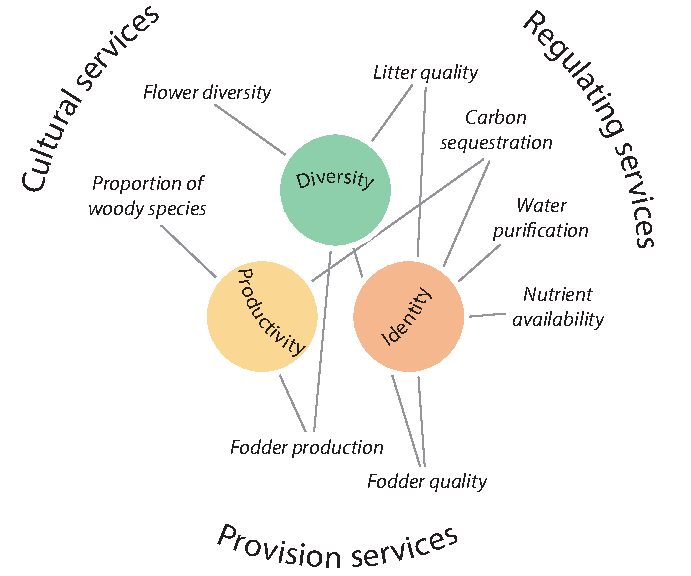
\includegraphics[width=1\linewidth]{./1_Introduction/graphics/services.pdf}
  \caption[Ecosystem services in mountain grasslands]{Classification of some of the ecosystem services provided by the mountain grasslands, linked to the main properties (circles) of the grassland communities. }
  \label{fig:services}
\end{figure}

Mountain grasslands provide numerous services that can be divided into multiple categories such as provision, cultural, and regulating services (see figure \ref{fig:services}). Provision services are related to the quantity and quality of primary resources the grasslands provide. Fodder production and quality are the main measures of provision services. Other services can be included in this category: diversity of flowers and phenology for flower and honey production for instance. Productivity is also relevant to assess carbon capture, a regulating service. Soil nutrient availability and water filtering are other regulating services impacted by the identity and diversity of species populating mountain grasslands. Finally, cultural services, related to tourism activity and landscape appeal are also related to grassland species diversity.


In case of terrestrial ecosystems, vegetation cover is often central because of its role in primary production, and the fact that vegetation community informs about the properties of the abiotic and biotic conditions. Moreover, most of studies on services from terrestrial ecosystem are interested in plants and soil invertebrates \cite{de_bello_towards_2011}, revealing the importance of vegetation in the provision of ecosystem services. In addition, in alpine habitats plant communities are susceptible to be the first impacted by global change because they cannot escape changes in conditions and are the target of management practices linked to fodder productions. All these arguments support the interest of studying the vegetation dynamics for the assessment of ecosystem services.


\paragraph{Properties}
Ecosystem services are tightly related to \textemph{ecosystem properties} (as illustrated in figures \ref{fig:services})\parencite{lavorel_predicting_2002, diaz_incorporating_2007} that can be extracted from a description of the grassland communities. Ecosystem properties are features of the community that characterise it and arise from the characteristics of all parts of the system or how they combine. The main properties of a plant community are captured in the following concepts:

\begin{itemize}
\item \textemph{identity}: the identity of the community refers to its community's dominant species (or directly its characteristics) that transfers its traits to the whole community. It can also refer to mean traits (with community-weighted mean measures) of a community. In this document, identity will often be used to talk about the resource-use strategy (\textit{i.e.} whether it is more or less exploitative. The term \textemph{exploitative} designates species that have rapid growth and lower resource use efficiency.)\parencite{grime_evidence_1977}. While this notion can encompass multiple traits and measures, it is practical to use one term to identify components of the community description that can be attributed to a species\sidenote{in opposition to variables that are related to a system, \textit{e.g.} diversity cannot be expressed for a species alone};

\item \textemph{diversity}: diversity plays a large role in the provision of multiple services, and is related to other properties of the community. Diversity can be expressed in term of species richness or functional diversity\sidenote{each measure depending on the functional space that is considered}, and by a wide range of indexes that are not discussed here. Despite a lot of nuances between these notions, they are often tightly correlated and diversity will be discussed in term of the number of species or functional volume\sidenote{volume of the space drawn by the functional traits of interest occupied by living species. It is a simple measure of the functional diversity. See \cite{laliberte_distance-based_2010} for alternative indexes.} in the rest of this document;

\item \textemph{productivity}: productivity captures the capacity of the system to produce organic matter in a given timespan. It is an ambiguous term as it can refer to the abiotic environment, to a species or a community property or even to a service. I will try to limit its use to the species or community vegetative biomass in a given condition.
\end{itemize}

%-----------------------------------------------------------------------------------------
%\subsection{From community description to ecosystem services: the facets of the community}

%Ecosystem services are various. Some of them can be easily assessed (e.g. fooder production and quality), while others are more subjective (cultural or recreational services) or hard to measure (carbon sequestration, water purification etc...). But all of them rely on a good description of the system, even though this description does not have to be complete as some aspects of an ecosystem might not be relevant to all provided services.


Linking ecosystem services to ecosystem properties is essential both for the understanding of processes controlling these services and for an easier quantification of such services. This is particularly important for the prediction of service levels to plan management practices in the context of global change. Some ecosystem services are linked to the main community properties as illustrated in figure  \ref{fig:services}. Because services are hard to assess, ones can take advantage of this link and assess levels of ecosystems services based on a detailed description of the community; of both its structure and properties. The structure is defined by the relative abundance of the different species of the community, and properties result from the combination of the structure and the specific characteristics of present species. Multiple drivers affect the relative abundance and characteristics of a given species, from abiotic filtering processes to biotic interactions. Thus, ecosystem services also largely depend on abiotic factors \parencite{lavorel_predicting_2002}. Therefore, there is a tight link between drivers, community structure and properties, and ecosystem services (see figure \ref{fig:drivers}) that can be exploited to predict changes in ecosystem services \parencite{lamarque_plant_2014}. 


\begin{marginfigure}
    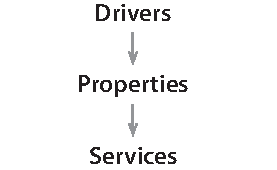
\includegraphics{./1_Introduction/graphics/drivers_properties_services_m.pdf}
  \caption[Drivers to services]{Link between abiotic drivers, community properties and ecosystem services.}
  \label{fig:drivers}
\end{marginfigure}

%The assessment of ecosystem services relies on a detailed characterisation of the community structure and properties. The knowledge of species characteristics and relative abundance allows the computation of summary variables that characterise the plant community. A long history of plant study and description gives us a good knowledge of benefit provided by specific species. 

%

%Need of mechanisms to produce dynamics and give properties.

%\textbf{The complexity of plant community dynamics requires mechanistic approaches to understand and predict system properties in new, extreme, and variable conditions. }


\textbf{The evaluation of ecosystem services relies on a precise description of an ecosystem's abiotic and biotic properties. In mountain ecosystems, the plant community is arguably the most dynamic and complex driver of ecosystem services, but direct links can be drawn between a fine description of the community and ecosystem services. Understanding and prediction the main dynamics that capture those links is necessary to efficiently predict changes in levels of ecosystem services.}

\textbf{Plant communities are complex interconnected systems. In order to evaluate ecosystem services, they can be summarised by three main types of variables that capture different dimensions of such systems: the diversity, the productivity, and the identity. %But grassland communities are natural systems driven by environmental variables, and changes in these drivers can lead  to changes in services because of this link.
}



\subsection{Global change: what changes and what consequences}

Mountain grasslands are maintained by strong climatic constraints that limit growth rate and lifeforms  \parencite{koorner_alpine_2003}, but also by frequent grazing or cutting perturbation regimes that strongly limit the growth of woody species and favour low stature species or rapid growth herbs \parencite{diaz_plant_2007}. But these drivers are changing at alarming rates with negative consequences on levels of ecosystem services \parencite{schroter_ecosystem_2005}. Moreover, mountain grasslands are suspected to be very vulnerable \parencite{schroter_ecosystem_2005, engler_21st_2011} due to higher variations in water availability regimes and specific warming processes \parencite{mountain_research_initiative_edw_working_group_elevation-dependent_2015}, stronger isolation (island effect due to rise in temperature) and reduction of the grazing pressure.

\paragraph{Climate change}

The rise of carbon dioxide in the atmosphere due to human activities has a large impact on climate. The constant increase in mean temperature is the best known and easily observable phenomenon (see figure \ref{fig:climate}). But mountain grasslands will also experience more frequent and severe drought event as well as precipitation events \parencite{beniston_climate_1997, solomon_climate_2007, intergovernmental_panel_on_climate_change_climate_2014}. Despite being relatively free from non native species, they are also predicted to experience longer growing seasons and stronger invasive pressure from alien species and species from a lower altitude \cite{alexander_plant_2016}.


\begin{figure}
    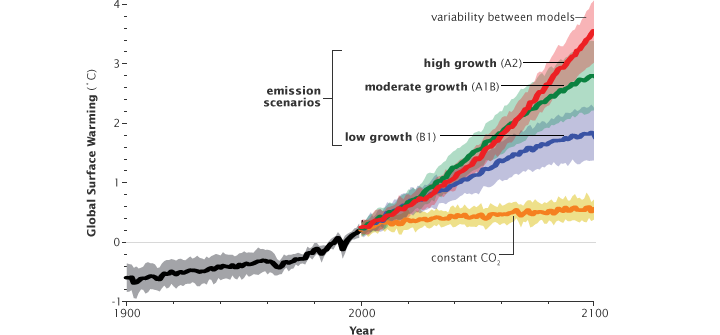
\includegraphics[width=1\linewidth]{./1_Introduction/graphics/ipcc_scenarios.png}
  \caption[IPCC scenarios for global mean temperature]{Historical models and projection scenarios for global mean temperature from \cite{solomon_climate_2007} }
  \label{fig:climate}
\end{figure}

%The changes in snowmelt, season length and drought event will certainly increase the range of conditions alpine plants will experience.
In this context, the ability of plants to adapt to such changes and to cope with new competitors, no more filtered out by climatic conditions, will greatly determine the response of alpine communities \parencite{alexander_novel_2015}.

\paragraph{Land-use mutations}

In addition to changes in climate, land use is also modified.  Land-use, mowing or grazing in alpine grasslands, is an important filter for slow-growing perennial species that try to accumulate biomass over multiple seasons. Because of such asymmetric effects, land-use acts as a strong driver and can cause mountain grassland communities to shift in dominant species, and thus along service gradients \parencite{schirpke_multiple_2013}. Land-use abandonment is suspected to greatly impact the invasion dynamics as it removes the pressure of biomass removal \parencite{carboni_simulating_2018}. 

\textbf{Global change is a source of considerable changes, both in mean regimes, but also frequency and amplitude of climatic events. In addition to changes in the climatic environment and resource availability, changes of management of mountain grasslands will also affect community dynamics and particularly competition hierarchies. These modifications of strong drivers will have large effects on plant communities, and therefore on the attributes and the services they provide.}

\textbf{Mountain grasslands provide numerous services that can be assessed thanks to main attributes of the plant community. But global change threaten these systems, and as consequence, the ecosystem services we take benefit of. We need tools to anticipate the effects of global change on these services and eventually adapt the management of mountain grasslands.}
%trade-off lavorel and 
%
%management change the position along these trade-offs
%
%climate also change things



 
%
%\section{Community dynamics: complexity emerging from parts and the role of phenotypic plasticity}
%title too vague to bring meaning should put both parts together.
\section{The need for new mechanistic models}


\subsection{The limit of classic patterns}
\paragraph{A new world}

The world is changing at a fast rate , but most importantly in ways never experienced by living species in recent history\parencite{butchart_global_2010, intergovernmental_panel_on_climate_change_climate_2014}. So, anticipating the effects of new environmental conditions on vegetation community cannot be built on the observation of previous or existing states. Extrapolation of complex system behaviour is considered to not be a good predictor of its current behaviour. The complexity of the prediction goes beyond the multiplicity of dimensions impacted by the global change (rising mean temperature, frequency, and amplitude of drought events, reduction of cutting frequency or grazing abandonment, etc...), as the drivers often interact, with positive or negative feedbacks. 

 \paragraph{Find balance}
 
 
 %community responses: different processes (recruitment, growth, plasticity etc...) \& levels (indiv, pop, metacommunity)
 
 To answer this challenge, large-scale experiments are conducted such as the Cedar Creek experiment in the United-States, or the JENA experiment in Germany. These experiments give high-value experimental data for various conditions and a variety of species, where interactions can be studied as well as management effects. Transplant experiments are also conducted to investigate the effects of temperature rise on the productivity, diversity, and identity of the community (as an example for SLA response see \cite{scheepens_genotypic_2010}, or  \cite{debouk_functional_2015} for an increase in productivity and decrease in diversity, as well as a shift toward more acquisitive species).
 
 But these common garden or transplant experiments also show contrasting responses, that can come from opposite responses between the intra-specific level and the inter-specific level \parencite{jung_intraspecific_2014}, between low and high elevation (changes in identity and contrasting effect in diversity between altitudes, observation data in \cite{rosbakh_elevation_2014}) or between effects (see effect of warming and carbon dioxide on phenology in \cite{reyes-fox_five_2016}).
 
 To accurately predict the future dynamics of grasslands communities, we need to be able to find the balance between dominant drivers that structure these ecosystems. It may also requires to identify eventual the interactions between those. For such complexity, empirical studies provide required and fundamental knowledge of processes and basic differences between effects, but no consensus can be made \parencite{merila_climate_2014} and additional approaches need to be developed and used.
 
 An additional argument for the use of alternative approaches is the uncertainty around climate scenarios (see figure \ref{fig:climate}). Indeed, the future of the atmosphere, and by consequence climate, depends mainly on how we humans are capable of changing our dependency on fossil energy \parencite{intergovernmental_panel_on_climate_change_climate_2014}. The will to adjust management scenarios to the future of vegetation community \parencite{schirpe_multiple_2013} also require extensive experiementation \parencite{rodriguez_lingra-cc:_1999, martin_simulations_2012, deleglise_drought-induced_2015}.
 
 
 
\begin{figure*}
    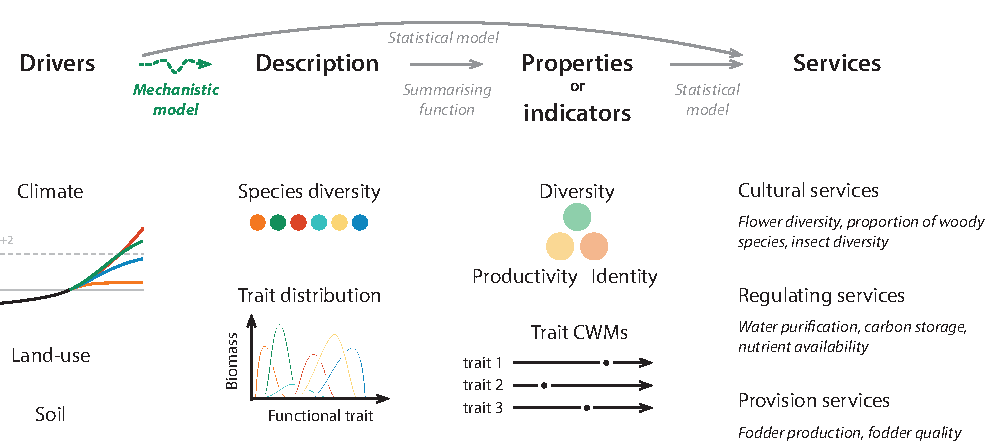
\includegraphics[width=1\linewidth]{./1_Introduction/graphics/drivers_to_services.pdf}
  \caption[From drivers to ecosystem services]{From drivers of community dynamics to ecosystem services. The effects of main drivers (climate and land-use) on grasslands dynamics is captured by mechanistic approaches to predict the composition and structure of the community. This description can then be used to assess the levels of ecosystem services through statistical models, to evaluate climatic scenarios or alternative land-use practices.}
  \label{fig:drivers2services}
\end{figure*}

Mechanistic approaches allow better linking of drivers with community dynamics. This link can then be used to assess levels of ecosystem services as illustrated in figure \ref{fig:drivers2services}\parencite{bello_towards_2010, lavorel_using_2011}.

%niche vs process: stronger effects predicted by niche based because of no plasticity or local adaptation \cite{morin_comparing_2009}



\subsection{When phenotypic plasticity makes things complicated}

Within the context of climate change, the ability of species to adapt has a great influence on the response of the community. Indeed, the capacity of species to adjust to variations in drivers, via genetic variability and mutations, or thanks to plastic mechanisms, will certainly buffer the response of the community to changes in climate or land-use. \cite{morin_comparing_2009} highlight stronger responses to climate change from vegetation communities within niche-based distribution models than within process-based models that capture adaptation mechanisms. More mechanistic processes should be included in these approaches \parencite{evans_towards_2016} to take into account adaptation mechanisms and interactions between species \parencite{gilman_framework_2010}. Plasticity can also change the competition intensity that increases negative effects of climate change  \parencite{hanel_phenotypic_2015}, while it can in other cases shift interactions from competition to facilitation  \parencite{callaway_phenotypic_2003}.

Phenotypic plasticity adds another level of complexity to the dynamic of communities and the interacting drivers. Statistical or expert based prediction cannot easily handle such complexity and mechanistic approaches have great potential to model complex systems.
%The question of adaptation is closely related to intra-specific variations as an intra-specific variation, whether genetic or plastic, are often justified by adaptation mechanisms (selection or adaptive plasticity).


%plus ignored effects of intra-specific variations: additional level of response: amplification or mitigations, driver dependencies?


\subsection{The rise of individual-based approaches}


\textemph{Individual-based-models} (IMBs) let the complex behaviours of systems composed of numerous interacting agents emerge from individual functioning. This type of modelling is extremely well adapted to the modelling of plant communities as we have a fairly good understanding of plant functioning, and parameters are relatively easy to measure. The dynamics of essential resources is also relatively easy to compute. Yet, this apparent simplicity is relative (to animal modelling for example) and numerous models have been developed with various simplification hypotheses. Most of these hypotheses deal with the essential resources: light is often ignored in grasslands, while forest models focus on this aspect of resource competition. The choice of model simplifications depends on the focus of the modelling exercise, and the importance of the given variables for the dynamics of the system.

\paragraph{Between climate and land-use}
These IBMs of plant communities have been used to investigate the effect of climate change in the study of \cite{rodriguez_lingra-cc:_1999} with the model LINGRA-CC and show an increase in productivity with predicted climate change. But such analysis is not decoupled from the land-use practicies, and in this example, the increase in productivity is shown to allow a higher cutting frequency. Alternative scenarios are also explore in other grassland models that take advantage of the mechanistic approach of the model to predict properties of the communties under different conditions or management scenarios \cite{taubert_review_2012, taubert_modelling_2014, maire_plasticity_2013, maire_trade-off_2009}. Forest modelling present also numerous implementations of individual-based models based on mechanistic functioning and trade-offs to better understand the drivers structuring diverse communities (see \cite{ falster_plant:_2016, marechaux_individual-based_2017} for recent forest model examples).

Other models based on processes can be used to study long terms dynamics in the context of climate change in mountain ecosystems. It can be used to study patterns of diversity \parencite{isabelle_fate-hd:_2014} or the impact of evolutionary processes on adaptation to climate change \parencite{cotto_dynamic_2017}.
 %an
% to test gc effect on productivity: higher productivity allowing shorter intervals between cutting


%Maire

%Lohier: vegetative phase, coexistence, and ontogeny... 

%Taubert: diversity productivity 


\subsection{Gaps to fill: plasticity}

A wide range of models has been developed to better understand biological processes involved in plant growth and population dynamics and the impact of climate change and land-use on these dynamics. They spread from organ-based models to functional types approaches. As the scale increases, the resolution diminishes and the verticality of processes is rarely taken into consideration. This is rarely a problem in stable conditions because the lower levels are implicitly integrated into the grain of larger processes (like the leaf gas exchanges regulation processes are ignored at the scale of the population). But two aspects can limit such simplification: (1) if the process is ignored instead of being integrated into higher level function (\textit{e.g.}: stomatal regulation is often not modelled because it is assumed that it is correlated to photosynthetic activity, either because it is limiting the photosynthesis when the vapour pressure deficit is high, or it is down-regulated to avoid water loss when photosynthesis is limited by other factors). However, phenotypic plasticity is often ignored but not translated into the hypotheses of the model. Moreover, variables that are directly impacted by this process are explicitly represented (unlike stomatal conductance with stomatal regulation processes) leading to a misrepresentation of these variables (especially root:shoot ratio (RSR) or strategic traits like SLA); (2) if the non-modelled process has a great impact on the dynamic of the system. 

\paragraph{Dichotomy between models}
Among models that target grasslands ecosystems  there is a dichotomy between growth models that are mainly interested in individual processes and species dynamics \cite{soussana_gemini:_2012, taubert_modelling_2014, lohier_analyse_2016}, and models interested in species-level processes and community dynamics \parencite{boulangeat_fate-dh_2014, cotto_dynamic_2017}. The former focus on the individual growth of a limited number of species. They take into account fine-scale resource dynamics and interactions driven by explicit strategies and precise plant functioning. These models are on the side of the spectrum of the development models that often focus on a single species. The productivity of the system is often the primary concern and questions relative to the management of these systems are privileged over questions concerning climate change (but see \cite{rodriguez_lingra-cc:_1999}, but still with the perspective of productivity). The latter is more interested in larger scale dynamics driven by the climate and evolutionary processes. The questions investigated with these models are therefore more often relative to climate change and adaptive dynamics of the communities and the effects on community diversity and identity. These models are closer to dynamic global vegetation models (DGVMs \sidenote{model at large scale that regroup plant species into wide functional groups and analyse large-scale dynamics. See \cite{kleidon_global_2000} for an example.}) despite finer scale interactions. This dichotomy highlights the lack of integrative models that support community dynamics at long time scales with modelling of processes at the individual scale, based on explicit resource dynamics. The explicit modelling of the link between plant strategies, plant functioning, resource dynamics and plant growth allows a solid integration of plant interaction and external drivers (via the effect of resource dynamics and plant growth). Moreover, phenotypic plasticity can be integrated at the plant level, while its complex effects are emergent. Finally, considering the growth of individuals, the strategies of species and the dynamics of the population is required to predict main facets of mountain grasslands communities (diversity, productivity, and identity) that can integrate both management practices and climate scenarios.

\paragraph{Where is the diversity}
Because models have often practicality objectives, it is easier to develop a model that can be calibrated with species-specific empirical data. They can also be calibrated with Bayesian procedures and pattern-based approaches \cite{hartig_statistical_2011}. As a consequence, these models often integrate a limited number of species or functional types. This requirement of calibration limits the number of species simulated. To model diverse communities and evolutionary processes, this species diversity is required and a generic framework is an attractive solution to avoid the calibration of individual species. Such high species diversity is observed in DGVMs that integrate trade-offs and multiple strategic axis \parencite{kleidon_global_2000, pavlick_jena_2013}.

\paragraph{Building bridges}
Mechanistic models are great tools and can be used to explore the uncertain future of mountain grasslands ecosystems. Bridges between individual-centred and generic community dynamics approaches must be built to take into account the complexity of population dynamics emerging from fine-scale interactions and plant functioning, driven both by environmental conditions and species strategies. Considering both levels is compulsory to capture the complexity of responses of vegetation communities exposed to diverse drivers.

%
%But 2 things:
%(1) ok to not explicitly represent if know and considered within a broader mech (translated into assumptions: \textit{e.g.}: assumption that stomata regulation), it is not the case of phenotypic plasticity as it is not considered in basic assumptions made. Plus, it depends on the scale, but daily growth require plasticity, period.
%(2) they may greatly change plant and community behaviour in changing conditon/environment.
%% 
%scales and processes (climate, management etc...)
%put the resoure in the center (fate-hd)
%
%process and mechanisms
%\parencite{berger_competition_2008}: effect on local env., adaptive beh, below-ground.
%partly filled (maire and Lohier).
%
%but lack of species diversity and genericity. 

%
%
%
%\section{Global change and community dynamics in alpine grasslands}
%\begin{figure*}
%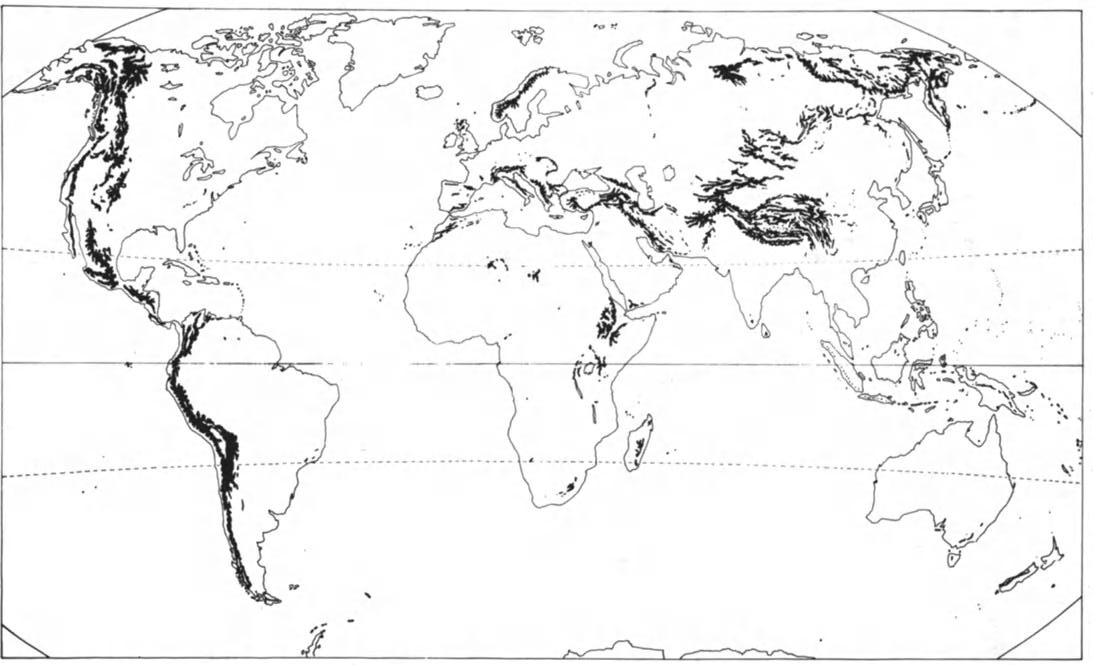
\includegraphics{./1_Introduction/graphics/alpine_distribution.jpeg}
%\caption{Distribution of alpine habitats}
%\end{figure*}
%
%Climate change is probably the greatest challenge the humanity has to face this century. Expected drastic changes in both average climatic conditions and punctual climatic event frequencies and intensities will, and already have, an impact all around the globe on multiple aspects of our lives. From agricultural and economic, to social and political, but also scientific and technical, the problems for human societies are numerous and multidimensional.\\ 
%Need to better understand and predict natural systems. Mountain grasslands are susceptible to be greatly impacted (even if certain think they might not). And in new ways as the rising temperature will certainly lead to migration to higher altitude, increasing the island characteristic of alpine habitats and reducing links between communities, and at the same time increasing the opportunity of invasion by lower altitude higher temperature species.\\
%\indent Detail a bit the characteristic of mountain grasslands, (snow, islands, grazing) the effect on species (snow-bed species, link to meta-community, diversity, species adaptation to frost etc... and how global change may affect that.\\
%\indent Because of that mountain grasslands are rich in species, but also vulnerable, that is why in parallel of predicting climate change, we also need to understand ecological mechanisms under this diversity and how they can be affected by global change \sidenote{section \ref{sec:coexistence}}. A key part in community diversity and in adaptation of communities also lies in the diversity and adaptation of individuals, so we are interested in intra-specific diversity and phenotypic plasticity \sidenote{section\ref{sec:intraspe}}.
%
%
%%Take home message ####################################
%\textbf{There is a need for new tools to predict the response of ecosystems to new climate conditions and management scenarios. These tools should integrate the complexity of such system and the mechanisms underlying the dynamic responses of these communities.}
%
%\section{Empirical results, trait approaches and need for a new kind of model in grasslands}
%
%\subsection{On trait-based approaches}
%
%Holy Graal of ecology\\
%Lavorel, Kraft, Kunstler
%
%\subsection{The importance of intra-specific variability}
%
%Jung
%Leps
%Albert
%Kichenin
%Lavorel (hypothesis of traits bell shape)
%Violle ...
%
%%Take home message ####################################
%\textbf{Trait approaches allow for generalisation and more direct link with processes and services. However they ignore variations and processes at lower levels than the species that are of critical importance for the understanding of community dynamics. A mechanistic approach integrating processes at the individual level and rich community complexity are needed.}
%
%\section{Close a gap in grassland modelling}
%
%%Take home message ####################################
%\textbf{Generalizing models for forest ecosystems and complex individual level models for grasslands coexist, but there is a need for a generalizing model at individual scale for grassland communities.}
%
%\section{Effect of phenotypic plasticity on coexistence and community dynamics}
%
%%Take home message ####################################
%\textbf{Despite empirical and theoretical work, the effects of intra-specific variability and plasticity on community dynamics are not fully disentangled. Understanding the effect of individual variations on plant community is crucial and may greatly alter how we envision the future of these ecosystems.}
%
%%_________________________________________________________________________________
%

\chapter{Aims, Objectives, and Overview}


\section{Aims: understanding and prediction}

Global change is probably the biggest challenge humanity has to face at the beginning of this millennium. Actions are urgently needed to reduce the release of carbon dioxide but also to mitigate the effect of climate change on natural and semi-natural systems. While solutions for the former must be found in technology, economics, and sociology, ecology can help with the latter. But it requires an understanding of how the drivers impacted by global change will impact these ecosystems. The multiplicity of environmental drivers impacted by global change - whose effects can synergise or balance themselves -, in addition to complex structure and dynamics of natural systems make this understanding hard to build and to summarise.

To go beyond traditional pattern-driven ecology and overcome the difficulty of combined causes leading interacting effects, mechanistic approaches are promising. 

The functioning of individuals living in these communities and the dynamics of the resources should be at the core of the new approaches to better understand the trajectories of the ecosystems.

%
%Functioning
%Diversity of : drivers, mechanisms, species, and strategies
%Flexibility: structure: genericity, experiments, plasticity

\section{Objectives: a new agent-based model for plant community dynamics} % the why
Traditional empirical approaches of observation and controlled experiments provided valuable information on the functioning of grassland ecosystems. However, they lack the power to quantitatively explore the consequences of the intricate interplay of the multiple processes, especially in case of uncertain scenarios.
%understand intricate systems and predict their dynamics, especially in case of uncertain scenarios. 

Modelling approaches must be used to build understanding and predictions of natural ecosystems dynamics driven by changing environmental drivers. These models should include a diversity of drivers as well as the diversity and the intrinsic complexity of these systems.

In order to compensate a long development time and to extend the reach of simulation experiments, models should try to be generic in structure and flexibility at use, while being specialisabled thanks to parameters or simple equation changes.

\subsection{Generic framework for multi-species and plastic plant modelling} % the how

In the context of mountain grasslands, showing unique levels of diversity despite strong environmental drivers, species diversity cannot be ignored to predict the response of the community. This diversity must be translated into species-specific functioning differences leading to diversity in niches and possible responses. In addition to species level dynamics driven by these differences, intra-specific responses cannot be ignored, and a phenotypic plasticity mechanism is needed.



%trade-off that constrain inter and intra differences in the same way

\subsection{Effect of phenotypic plasticity on plant growth, community properties, and dynamics}

Intra-specific variations are expected to play an important role in the response of mountain grassland communities to global change. Disentangling the effects of the different sources of intra-specific variability can help us understand and predict their specific roles in the grassland dynamics. The explicit integration of species-specific phenotypic plasticity in a plant community model can help identify the specific consequences of this process and understand its effects.

As multiple services derive from the main properties of the vegetation of mountain grasslands, it is crucial to establish how phenotypic plasticity specifically impacts these properties. Because these properties depend both on properties of the individuals and the relative abundance and diversity of species, effects on processes at both individual and community scales should be investigated.


\section{Thesis overview}

The rest of this thesis is divided into five chapters. The following chapter \ref{part:literature}, in the form of a literature review, introduces the concepts and knowledge that support the approach developed in later chapters. The chapter \ref{part:model} develops the generic framework for plant functioning and phenotypic plasticity from the concepts established in chapter \ref{part:literature}. Chapters \ref{part:individuals} and \ref{part:community} present respectively individual and community scale results of simulations made with the developed model \model on the effects of phenotypic plasticity on main plant community properties. The final chapter discusses the outcomes of this work and possible paths to follow from the presented conclusions. Further model developments are also proposed.


\begin{figure*}
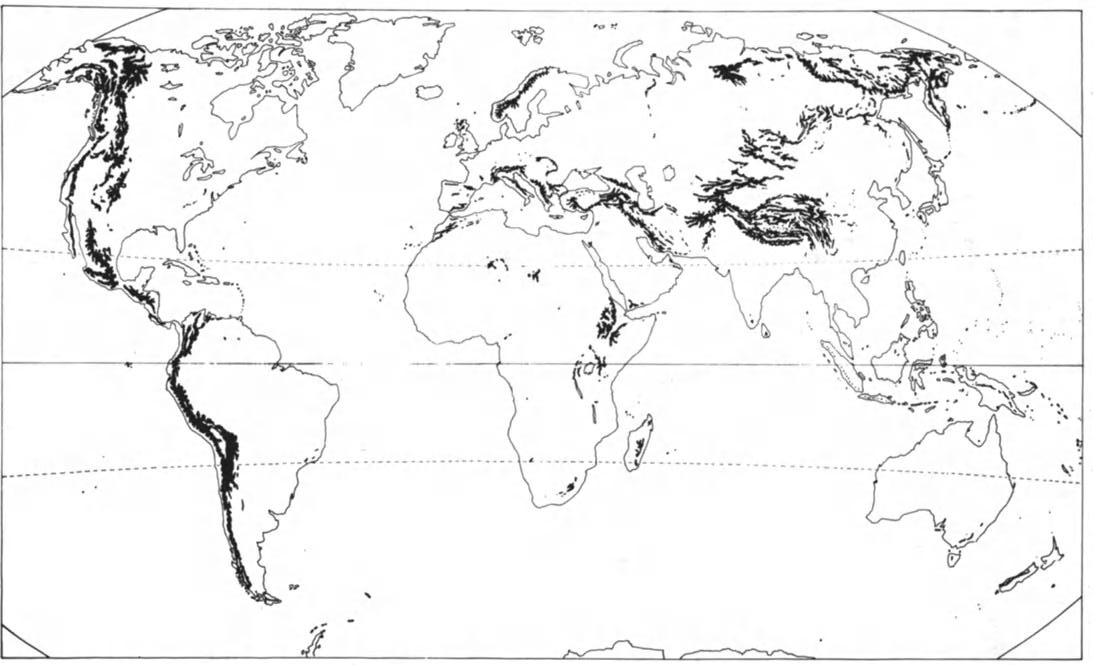
\includegraphics{./1_Introduction/graphics/alpine_distribution.jpeg}
\caption{Distribution of alpine habitats. Alpine habitats shelter unique and rich ecosystems providing numerous services to human populations. Climate change and mutations of land-use practices threaten these dispersed and fragile habitats. From \cite{korner_alpine_2003}, reproduced with the permission of Springer, license number: 4384831420904.} \label{fig:distribution}
\end{figure*}
